\documentclass[10pt]{article}
\usepackage{a4wide}
\usepackage[english]{babel}
\usepackage{graphicx}
\usepackage{tabu}
\usepackage{textcomp}
\usepackage{fancyhdr}
\usepackage{lastpage}
\usepackage{titlesec}
\usepackage{lscape}
\usepackage{longtable}
\usepackage{color}
\usepackage{listings}
\usepackage{xkeyval}

\definecolor{mygreen}{rgb}{0,0.6,0}
\definecolor{mygray}{rgb}{0.5,0.5,0.5}
\definecolor{mymauve}{rgb}{0.58,0,0.82}

\lstset{ % Syntax highliughting for java
    backgroundcolor=\color{white},   % choose the background color; you must add \usepackage{color} or \usepackage{xcolor}
    basicstyle=\footnotesize,        % the size of the fonts that are used for the code
    breakatwhitespace=false,         % sets if automatic breaks should only happen at whitespace
    breaklines=true,                 % sets automatic line breaking
    captionpos=b,                    % sets the caption-position to bottom
    commentstyle=\color{mygreen},    % comment style
    deletekeywords={...},            % if you want to delete keywords from the given language
    escapeinside={\%*}{*)},          % if you want to add LaTeX within your code
    extendedchars=true,              % lets you use non-ASCII characters; for 8-bits encodings only, does not work with UTF-8
    frame=none,                    % adds a frame around the code
    keepspaces=true,                 % keeps spaces in text, useful for keeping indentation of code (possibly needs columns=flexible)
    keywordstyle=\color{blue},       % keyword style
    language=Octave,                 % the language of the code
    morekeywords={*,...},            % if you want to add more keywords to the set
    numbers=left,                    % where to put the line-numbers; possible values are (none, left, right)
    numbersep=5pt,                   % how far the line-numbers are from the code
    numberstyle=\tiny\color{mygray}, % the style that is used for the line-numbers
    rulecolor=\color{black},         % if not set, the frame-color may be changed on line-breaks within not-black text (e.g. comments (green here))
    showspaces=false,                % show spaces everywhere adding particular underscores; it overrides 'showstringspaces'
    showstringspaces=false,          % underline spaces within strings only
    showtabs=false,                  % show tabs within strings adding particular underscores
    stepnumber=5,                    % the step between two line-numbers. If it's 1, each line will be numbered
    stringstyle=\color{mymauve},     % string literal style
    tabsize=4,                       % sets default tabsize to 2 spaces
    title=\lstname                   % show the filename of files included with \lstinputlisting; also try caption instead of title
}
%%%%%%
%% Variables for version and release status
%% useage: \version
%%%%%%
\newcommand\module{CS23710}
\newcommand\moduleName{Counting the Cetacean Mammals of Cardigan Bay}
\newcommand\authorText{Nicholas Dart}
\newcommand\authorUsername{nid21}
\newcommand\studentID{130057750}
\newcommand\assesser{Some prof}

%%%%%%
%% Alias
%%%%%%
%% \newcommand{\sectionbreak}{\clearpage}  %% Allways start a section on a new page


%%%%%%
%% Alias
%%%%%%
%\newcommand{\sectionbreak}{\clearpage}    %% Allways start a section on a new page
%% Never worked anyway...
%% ]\newcommand{\figureRef[x]{i}{d}{l}}{\begin{figure} \centering \includegraphics[scale=x]{i} \caption{d} \label{fig:l} \end{figure}}

\title{ \huge \module Assignment \\ \Large \moduleName}
\author{
    \vspace{100pt}
    \begin{tabular}{ r || l }
        Author          & \authorText (\authorUsername)\\
                        & \studentID \\
        Date Published  & \today \\
                        & \\
        Assessed By     & \assesser \\
        Department      & Computer Science \\
        Address         & Aberystwyth University \\
                        & Penglais Campas \\
                        & Ceredigion \\
                        & SY23 3DB \\
    \end{tabular} \\
    Copyright \textcopyright Aberystwyth University 2014
    %get rid of the date on the titlepage
    \date{}
}

\pagestyle{fancy}
\fancyhf{}
\lhead{\module~Assignment}
\rhead{\authorText~-~\studentID}
\rfoot{Page \thepage \hspace{1pt} of \pageref{LastPage}}
\lfoot{Aberystwyth University - Computer Science}

\begin{document}
    \setcounter{page}{1}

    \maketitle
    \thispagestyle{empty}
    \clearpage

    \tableofcontents
    \clearpage

    \section{Introduction}
        In this project, we are to make a C program, running on a common UNIX operating system, that can achieve the following tasks:

        \subsection{Feature One}
            Feature one must read in data from an observers and a sightings text files as described in section \ref{sec:observersFile} and \ref{sec:sightingsFile}. The data from these two text files must then be combined to create an mammal sighting with an absolute location in the world. This sighting should continue to contain data about who saw it and their positions. These absolute sightings should then be printed out for the user.
        \subsection{Feature Two}
            Feature two must take the absolute sightings from feature one and determine unique sightings. A sighting is considered non-unique if it is within \texttt{0.02} nautical miles from another sighting of the same type. This can be the case for several sightings. If multiple sightings are found to be within this range, then their positions are to be averaged out to produce one unique sighting.
        \subsection{Feature Three}
            Feature three then uses these unique sightings to determine if there are any \texttt{pods} in the area. A pod is defined as a sighting within \texttt{0.1} nautical miles of another sighting. The program should then collate these unique sightings into a pod and print the pod and it's sightings.

        \subsection{Input files}
            \subsubsection{Observers}
                \label{sec:observersFile}
                The observers file contains a list of observers, with an \texttt{ID} associated to them, a \texttt{Longitude} and \texttt{Latitude} in degrees as is common with nautical positioning. The file also contains a date and time at the beginning of the file. An example is provided below:
                \begin{verbatim}
                    01 01 2014 13 00 00
                    AA00 51.921867 -3.517409
                    ...
                \end{verbatim}

            \subsubsection{Sightings}
                \label{sec:sightingsFile}
                The sightings file contains a list of sightings from the observers. A sighting has an associated \texttt{observer}, a character to represent \texttt{type}, and a \texttt{bearing} and \texttt{range} from the observer. An example is provided below
                \begin{verbatim}
                    AA00 P 198.34981 0.301153
                    AA00 D 22.01652 3.985412
                    ...
                \end{verbatim}

    \newpage
    \section{Design Decisions}
        \subsection{Data Storage}
            A large part of this project was storing the data without duplicating it, and keeping it accessible between features. For this task i decided to use almost without exception \texttt{malloc} to allocate memory as needed, which has the advantage that this program should run with any sized data set. 

            \subsubsection{LinkedList}
                The task of grouping things together required a large amount of interconnection between data. C does not provide a way of making linked lists so I implemented my own. This was done to allow iterating through a collection of data and removing or inserting items seamlessly without gaps or having to move objects around in memory.

                I realized I needed a way to create LinkedLists dynamically at runtime so I have made a \texttt{struct} called \texttt{LinkedList} which contains a \texttt{headPointer} and a \texttt{tailPointer} to a \texttt{DataItem struct}. The \texttt{DataItem struct} is a generic \texttt{LinkedList} item that contains a \texttt{void*} pointer to an object. I chose to use \texttt{void*} pointers as it gives me freedom to use what ever item I need to. I could have encapsulated it better and had methods that cast the item to \texttt{Pod} or \texttt{Entity}, but I felt it wasn't used enough to require such functionality. 

            \subsubsection{Structs}
                I have made a \texttt{structs} for the two sources of data, each containing relevant fields for the data. I have then also made a \texttt{struct} for a ``definitive sighting''; a collection of sighting too close together to be considered unique. There is also a \texttt{Pod struct} which holds a list of ``definitive sightings''. Finally I have the aforementioned \texttt{LinkedList} and \texttt{DataItem structs} which hold data to be used in a list. 
                \begin{enumerate}
                    \item Sighting
                    \item Observer
                    \item Definitive Sighting
                    \item Pod
                    \item Linked List
                    \item Linked List Data Item
                \end{enumerate}

            \subsubsection{Sightings too Close Together}
                For feature 2, the specification requires sightings withing 0.02 nautical miles to be considered the same mammal. I realized that this allows for the possibility of a ``definitive sighting'' that contains a long line of sightings each within 0.02 nautical miles of the next. I felt this was not something that was desired and so have altered my program to group sightings if they are within 0.02 nautical miles of an average. This has a slight problem two ``distinct sightings'' could have sightings within 0.02 nautical miles of each other but belong to different ``distinct sightings''.

    \newpage
    \begin{landscape}
        \section{Netbeans screenshot}
            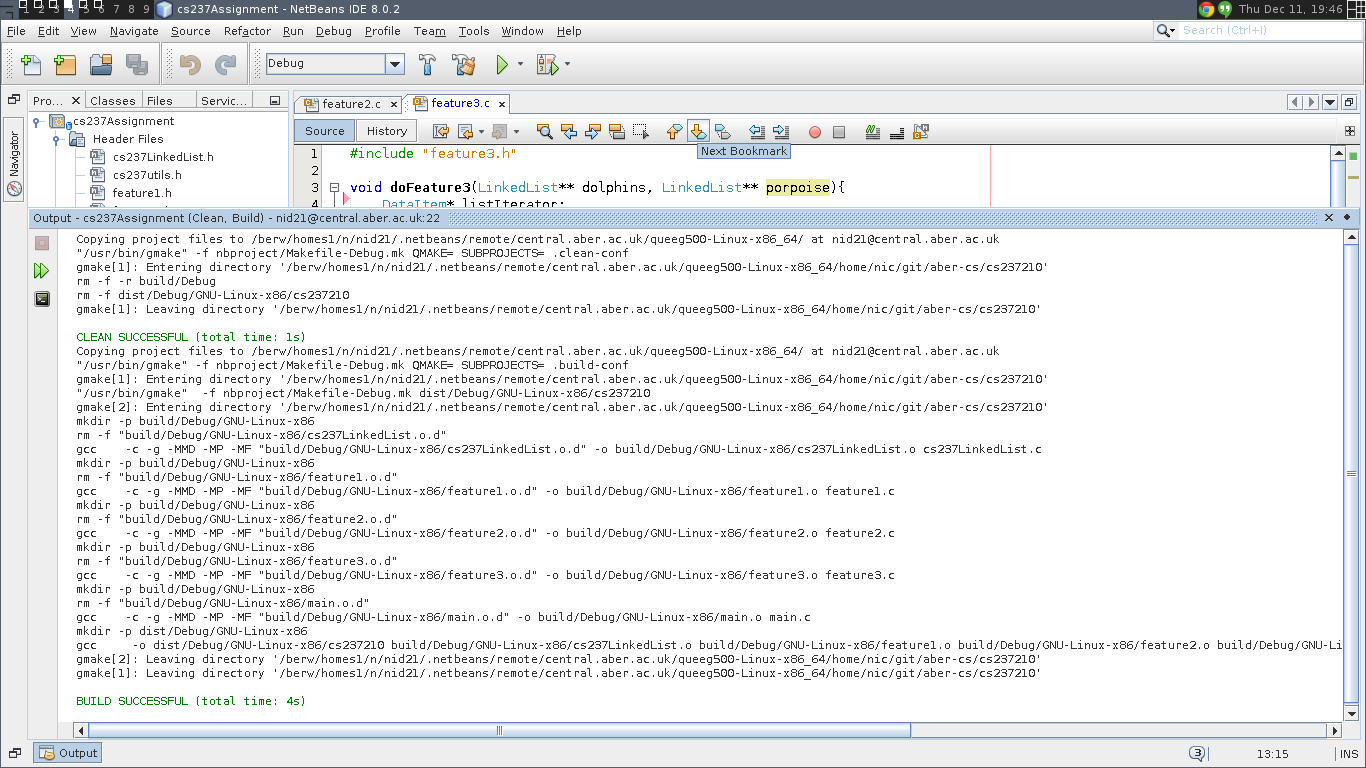
\includegraphics[scale=0.45]{netbeansOutput.png}
    \end{landscape}

    \newpage
    \section{Output}
        \subsection{Data Set 1}
            \begin{verbatim}
===== Entering Phase 1 =====
 >> Please enter observers file: >> observers_1.txt
05/11/2014 14:53:00
 >> Please enter sightings file: >> sightings_1.txt
UID     OLAT    OLNG    TYPE    BEARING RANGE   CMLAT   CMLNG
AB01    52.408  -4.217  P       270.0   4.100   52.408  -4.329
AB01    52.408  -4.217  D       275.0   4.500   52.415  -4.339
Found a sighting (51.837 lat, -4.417 long) out of bounds, Ignoring
Found a sighting (51.867 lat, -4.369 long) out of bounds, Ignoring
Found a sighting (52.030 lat, -6.135 long) out of bounds, Ignoring
Found a sighting (52.138 lat, -5.904 long) out of bounds, Ignoring
===== Entering Phase 2 =====
UID     OLAT    OLNG    TYPE    BEARING RANGE   CMLAT   CMLNG

AB01    52.408  -4.217  D       275.0   4.500   52.415  -4.339
AVRG    0.000   0.000   D       0.0     0.000   52.415  -4.339

AB01    52.408  -4.217  P       270.0   4.100   52.408  -4.329
AVRG    0.000   0.000   P       0.0     0.000   52.408  -4.329
===== Entering Phase 3 =====
UID     OLAT    OLNG    TYPE    BEARING RANGE   CMLAT   CMLNG
POD 1
AB01    52.408  -4.217  D       275.0   4.500   52.415  -4.339

POD 1
AB01    52.408  -4.217  P       270.0   4.100   52.408  -4.329

Found 2 Pods, 1 of Dolphins, 1 of Porpoises
===== Phase 3 Finished =====
            \end{verbatim}

        \newpage
        \subsection{Data Set 2}
            \begin{verbatim}
===== Entering Phase 1 =====
 >> Please enter observers file: >> observers_2.txt
24/11/2014 16:39:00
 >> Please enter sightings file: >> sightings_2.txt
UID     OLAT    OLNG    TYPE    BEARING RANGE   CMLAT   CMLNG
CB00    52.626  -5.175  P       20.2    0.152   52.628  -5.174
CB01    52.628  -5.175  P       96.1    0.057   52.628  -5.174
CB02    52.313  -5.167  P       151.3   1.546   52.291  -5.147
CB03    52.294  -5.161  P       111.8   0.565   52.291  -5.147
CB04    52.429  -4.260  D       174.6   0.355   52.423  -4.259
CB05    52.454  -4.299  D       141.8   2.353   52.423  -4.259
CB06    52.217  -5.409  D       64.4    2.043   52.232  -5.359
CB07    52.286  -4.489  P       42.3    2.313   52.315  -4.446
===== Entering Phase 2 =====
UID     OLAT    OLNG    TYPE    BEARING RANGE   CMLAT   CMLNG

CB04    52.429  -4.260  D       174.6   0.355   52.423  -4.259
CB05    52.454  -4.299  D       141.8   2.353   52.423  -4.259
AVRG    0.000   0.000   D       0.0     0.000   52.423  -4.259

CB06    52.217  -5.409  D       64.4    2.043   52.232  -5.359
AVRG    0.000   0.000   D       0.0     0.000   52.232  -5.359

CB00    52.626  -5.175  P       20.2    0.152   52.628  -5.174
CB01    52.628  -5.175  P       96.1    0.057   52.628  -5.174
AVRG    0.000   0.000   P       0.0     0.000   52.628  -5.174

CB02    52.313  -5.167  P       151.3   1.546   52.291  -5.147
CB03    52.294  -5.161  P       111.8   0.565   52.291  -5.147
AVRG    0.000   0.000   P       0.0     0.000   52.291  -5.147

CB07    52.286  -4.489  P       42.3    2.313   52.315  -4.446
AVRG    0.000   0.000   P       0.0     0.000   52.315  -4.446
===== Entering Phase 3 =====
UID     OLAT    OLNG    TYPE    BEARING RANGE   CMLAT   CMLNG
POD 1
CB04    52.429  -4.260  D       174.6   0.355   52.423  -4.259
CB05    52.454  -4.299  D       141.8   2.353   52.423  -4.259
POD 2
CB06    52.217  -5.409  D       64.4    2.043   52.232  -5.359

POD 1
CB00    52.626  -5.175  P       20.2    0.152   52.628  -5.174
CB01    52.628  -5.175  P       96.1    0.057   52.628  -5.174
POD 2
CB02    52.313  -5.167  P       151.3   1.546   52.291  -5.147
CB03    52.294  -5.161  P       111.8   0.565   52.291  -5.147
POD 3
CB07    52.286  -4.489  P       42.3    2.313   52.315  -4.446

Found 5 Pods, 2 of Dolphins, 3 of Porpoises
===== Phase 3 Finished =====

            \end{verbatim}

        \newpage
        \subsection{Data Set 3}
            \begin{verbatim}
===== Entering Phase 1 =====
 >> Please enter observers file: >> observers_3.txt
25/11/2014 17:18:00
 >> Please enter sightings file: >> sightings_3.txt
UID     OLAT    OLNG    TYPE    BEARING RANGE   CMLAT   CMLNG
CB00    52.497  -4.760  D       348.5   0.591   52.507  -4.764
CB01    52.472  -4.744  D       341.0   2.185   52.507  -4.764
CB02    52.452  -4.096  D       228.3   2.538   52.424  -4.148
CB03    52.470  -4.139  D       186.5   2.823   52.424  -4.147
CB04    52.531  -4.597  D       147.0   2.323   52.499  -4.562
CB05    52.467  -4.504  D       311.8   2.833   52.499  -4.562
CB06    52.410  -4.261  D       352.7   0.093   52.411  -4.261
CB07    52.524  -4.663  D       143.6   0.926   52.512  -4.648
CB08    52.530  -4.659  D       159.3   1.164   52.512  -4.648
CB09    52.426  -4.273  D       72.7    2.913   52.440  -4.197
CB10    52.445  -4.259  D       96.5    2.256   52.440  -4.197
CB11    52.672  -5.361  D       330.9   0.889   52.685  -5.373
CB12    52.374  -4.969  D       287.9   0.063   52.374  -4.970
CB13    52.079  -5.163  D       358.0   2.648   52.123  -5.166
CB14    52.123  -5.170  D       98.6    0.177   52.123  -5.166
CB15    52.427  -5.358  D       31.7    1.755   52.452  -5.332
CB16    52.680  -5.334  D       248.8   2.677   52.664  -5.402
CB17    52.668  -5.387  D       243.5   0.623   52.664  -5.402
CB18    52.177  -5.386  P       112.2   1.927   52.165  -5.338
CB19    52.148  -5.285  P       298.6   2.213   52.165  -5.338
CB20    52.433  -4.369  P       39.7    1.245   52.449  -4.347
CB21    52.438  -4.384  D       36.4    1.542   52.459  -4.359
CB22    52.295  -4.665  D       51.5    2.228   52.318  -4.618
CB23    52.481  -4.898  P       245.3   0.924   52.474  -4.921
CB24    52.475  -4.921  P       188.4   0.028   52.474  -4.921
CB25    52.462  -4.186  D       156.8   1.679   52.436  -4.168
CB26    52.415  -4.178  D       16.9    1.317   52.436  -4.168
CB27    52.338  -4.865  D       198.0   0.629   52.328  -4.870
CB28    52.545  -4.658  D       308.1   1.760   52.564  -4.696
CB29    52.562  -4.694  D       321.1   0.102   52.564  -4.696
CB30    52.200  -5.124  D       151.7   1.818   52.173  -5.100
CB31    52.174  -5.101  D       130.0   0.044   52.173  -5.100
CB32    52.526  -4.536  D       184.7   1.173   52.506  -4.539
CB33    52.345  -4.334  P       58.3    1.965   52.362  -4.288
CB34    52.366  -4.285  P       207.5   0.279   52.362  -4.288
CB35    52.400  -5.514  P       16.5    2.395   52.439  -5.495
CB36    52.437  -5.516  P       81.6    0.760   52.439  -5.495
CB37    52.212  -5.118  D       216.3   1.513   52.192  -5.143
CB38    52.405  -4.289  P       187.0   2.789   52.359  -4.298
CB39    52.360  -4.297  P       202.7   0.114   52.359  -4.298
===== Entering Phase 2 =====
UID     OLAT    OLNG    TYPE    BEARING RANGE   CMLAT   CMLNG

CB00    52.497  -4.760  D       348.5   0.591   52.507  -4.764
CB01    52.472  -4.744  D       341.0   2.185   52.507  -4.764
AVRG    0.000   0.000   D       0.0     0.000   52.507  -4.764

CB02    52.452  -4.096  D       228.3   2.538   52.424  -4.148
CB03    52.470  -4.139  D       186.5   2.823   52.424  -4.147
AVRG    0.000   0.000   D       0.0     0.000   52.424  -4.147

CB04    52.531  -4.597  D       147.0   2.323   52.499  -4.562
CB05    52.467  -4.504  D       311.8   2.833   52.499  -4.562
AVRG    0.000   0.000   D       0.0     0.000   52.499  -4.562

CB06    52.410  -4.261  D       352.7   0.093   52.411  -4.261
AVRG    0.000   0.000   D       0.0     0.000   52.411  -4.261

CB07    52.524  -4.663  D       143.6   0.926   52.512  -4.648
CB08    52.530  -4.659  D       159.3   1.164   52.512  -4.648
AVRG    0.000   0.000   D       0.0     0.000   52.512  -4.648

CB09    52.426  -4.273  D       72.7    2.913   52.440  -4.197
CB10    52.445  -4.259  D       96.5    2.256   52.440  -4.197
AVRG    0.000   0.000   D       0.0     0.000   52.440  -4.197

CB11    52.672  -5.361  D       330.9   0.889   52.685  -5.373
AVRG    0.000   0.000   D       0.0     0.000   52.685  -5.373

CB12    52.374  -4.969  D       287.9   0.063   52.374  -4.970
AVRG    0.000   0.000   D       0.0     0.000   52.374  -4.970

CB13    52.079  -5.163  D       358.0   2.648   52.123  -5.166
CB14    52.123  -5.170  D       98.6    0.177   52.123  -5.166
AVRG    0.000   0.000   D       0.0     0.000   52.123  -5.166

CB15    52.427  -5.358  D       31.7    1.755   52.452  -5.332
AVRG    0.000   0.000   D       0.0     0.000   52.452  -5.332

CB16    52.680  -5.334  D       248.8   2.677   52.664  -5.402
CB17    52.668  -5.387  D       243.5   0.623   52.664  -5.402
AVRG    0.000   0.000   D       0.0     0.000   52.664  -5.402

CB21    52.438  -4.384  D       36.4    1.542   52.459  -4.359
AVRG    0.000   0.000   D       0.0     0.000   52.459  -4.359

CB22    52.295  -4.665  D       51.5    2.228   52.318  -4.618
AVRG    0.000   0.000   D       0.0     0.000   52.318  -4.618

CB25    52.462  -4.186  D       156.8   1.679   52.436  -4.168
CB26    52.415  -4.178  D       16.9    1.317   52.436  -4.168
AVRG    0.000   0.000   D       0.0     0.000   52.436  -4.168

CB27    52.338  -4.865  D       198.0   0.629   52.328  -4.870
AVRG    0.000   0.000   D       0.0     0.000   52.328  -4.870

CB28    52.545  -4.658  D       308.1   1.760   52.564  -4.696
CB29    52.562  -4.694  D       321.1   0.102   52.564  -4.696
AVRG    0.000   0.000   D       0.0     0.000   52.564  -4.696

CB30    52.200  -5.124  D       151.7   1.818   52.173  -5.100
CB31    52.174  -5.101  D       130.0   0.044   52.173  -5.100
AVRG    0.000   0.000   D       0.0     0.000   52.173  -5.100

CB32    52.526  -4.536  D       184.7   1.173   52.506  -4.539
AVRG    0.000   0.000   D       0.0     0.000   52.506  -4.539

CB37    52.212  -5.118  D       216.3   1.513   52.192  -5.143
AVRG    0.000   0.000   D       0.0     0.000   52.192  -5.143

CB18    52.177  -5.386  P       112.2   1.927   52.165  -5.338
CB19    52.148  -5.285  P       298.6   2.213   52.165  -5.338
AVRG    0.000   0.000   P       0.0     0.000   52.165  -5.338

CB20    52.433  -4.369  P       39.7    1.245   52.449  -4.347
AVRG    0.000   0.000   P       0.0     0.000   52.449  -4.347

CB23    52.481  -4.898  P       245.3   0.924   52.474  -4.921
CB24    52.475  -4.921  P       188.4   0.028   52.474  -4.921
AVRG    0.000   0.000   P       0.0     0.000   52.474  -4.921

CB33    52.345  -4.334  P       58.3    1.965   52.362  -4.288
CB34    52.366  -4.285  P       207.5   0.279   52.362  -4.288
AVRG    0.000   0.000   P       0.0     0.000   52.362  -4.288

CB35    52.400  -5.514  P       16.5    2.395   52.439  -5.495
CB36    52.437  -5.516  P       81.6    0.760   52.439  -5.495
AVRG    0.000   0.000   P       0.0     0.000   52.439  -5.495

CB38    52.405  -4.289  P       187.0   2.789   52.359  -4.298
CB39    52.360  -4.297  P       202.7   0.114   52.359  -4.298
AVRG    0.000   0.000   P       0.0     0.000   52.359  -4.298
===== Entering Phase 3 =====
UID     OLAT    OLNG    TYPE    BEARING RANGE   CMLAT   CMLNG
POD 1
CB00    52.497  -4.760  D       348.5   0.591   52.507  -4.764
CB01    52.472  -4.744  D       341.0   2.185   52.507  -4.764
POD 2
CB02    52.452  -4.096  D       228.3   2.538   52.424  -4.148
CB03    52.470  -4.139  D       186.5   2.823   52.424  -4.147
POD 3
CB04    52.531  -4.597  D       147.0   2.323   52.499  -4.562
CB05    52.467  -4.504  D       311.8   2.833   52.499  -4.562
POD 4
CB06    52.410  -4.261  D       352.7   0.093   52.411  -4.261

POD 1
CB18    52.177  -5.386  P       112.2   1.927   52.165  -5.338
CB19    52.148  -5.285  P       298.6   2.213   52.165  -5.338
POD 2
CB20    52.433  -4.369  P       39.7    1.245   52.449  -4.347

Found 6 Pods, 4 of Dolphins, 2 of Porpoises
===== Phase 3 Finished =====

            \end{verbatim}

        \newpage
        \subsection{Data Set 4}
            \begin{verbatim}
===== Entering Phase 1 =====
 >> Please enter observers file: >> observers_4.txt
24/11/2014 16:39:00
 >> Please enter sightings file: >> sightings_4.txt
UID     OLAT    OLNG    TYPE    BEARING RANGE   CMLAT   CMLNG
Found a sighting (52.693 lat, -5.557 long) out of bounds, Ignoring
Found a sighting (52.693 lat, -5.557 long) out of bounds, Ignoring
Found a sighting (52.186 lat, -5.521 long) out of bounds, Ignoring
Found a sighting (52.186 lat, -5.521 long) out of bounds, Ignoring
CB04    52.391  -4.317  D       174.6   0.355   52.385  -4.316
CB05    52.416  -4.356  D       141.8   2.353   52.385  -4.316
Found a sighting (52.098 lat, -5.808 long) out of bounds, Ignoring
CB07    52.194  -4.612  P       42.3    2.313   52.222  -4.570
===== Entering Phase 2 =====
UID     OLAT    OLNG    TYPE    BEARING RANGE   CMLAT   CMLNG

CB04    52.391  -4.317  D       174.6   0.355   52.385  -4.316
CB05    52.416  -4.356  D       141.8   2.353   52.385  -4.316
AVRG    0.000   0.000   D       0.0     0.000   52.385  -4.316

CB07    52.194  -4.612  P       42.3    2.313   52.222  -4.570
AVRG    0.000   0.000   P       0.0     0.000   52.222  -4.570
===== Entering Phase 3 =====
UID     OLAT    OLNG    TYPE    BEARING RANGE   CMLAT   CMLNG
POD 1
CB04    52.391  -4.317  D       174.6   0.355   52.385  -4.316
CB05    52.416  -4.356  D       141.8   2.353   52.385  -4.316

POD 1
CB07    52.194  -4.612  P       42.3    2.313   52.222  -4.570

Found 2 Pods, 1 of Dolphins, 1 of Porpoises
===== Phase 3 Finished =====
            \end{verbatim}

        \newpage
        \subsection{Data Set 5}
            \begin{verbatim}
===== Entering Phase 1 =====
 >> Please enter observers file: >> observers_5.txt
05/12/2014 18:11:00
 >> Please enter sightings file: >> sightings_5.txt
UID     OLAT    OLNG    TYPE    BEARING RANGE   CMLAT   CMLNG
CB00    52.417  -4.176  P       198.3   2.301   52.381  -4.196
CB01    52.393  -4.193  P       186.8   0.757   52.381  -4.196
CB02    52.404  -4.215  P       151.3   1.546   52.381  -4.195
CB03    52.385  -4.209  P       111.8   0.565   52.381  -4.195
CB04    52.772  -5.343  P       222.6   2.682   52.739  -5.393
CB05    52.740  -5.401  P       102.4   0.303   52.739  -5.393
CB06    52.724  -5.443  P       64.4    2.043   52.739  -5.392
CB07    52.761  -5.355  P       225.5   1.853   52.739  -5.392
CB08    52.741  -5.407  P       97.5    0.560   52.739  -5.392
CB09    52.734  -5.420  P       72.6    1.102   52.740  -5.391
CB10    52.716  -5.371  P       334.0   1.628   52.740  -5.390
CB11    52.736  -5.403  P       60.5    0.513   52.740  -5.390
CB12    52.244  -4.417  P       300.3   0.246   52.246  -4.423
CB13    52.245  -4.417  P       277.3   0.223   52.246  -4.423
CB14    52.223  -4.440  P       24.9    1.537   52.247  -4.423
CB15    52.205  -4.459  P       28.1    2.894   52.247  -4.422
CB16    52.237  -4.394  P       300.1   1.178   52.247  -4.422
CB17    52.265  -4.494  P       112.0   2.865   52.247  -4.422
CB18    52.253  -4.428  P       145.5   0.417   52.247  -4.422
CB19    52.257  -4.421  P       180.2   0.579   52.248  -4.421
CB20    52.319  -5.454  D       339.2   0.864   52.332  -5.462
CB21    52.348  -5.497  D       127.2   1.578   52.332  -5.462
CB22    52.323  -5.459  D       348.5   0.591   52.333  -5.462
CB23    52.298  -5.442  D       341.0   2.185   52.333  -5.462
CB24    52.338  -5.469  D       132.8   0.402   52.333  -5.461
CB25    52.407  -4.144  D       231.6   1.831   52.388  -4.183
CB26    52.420  -4.217  D       147.0   2.323   52.388  -4.183
CB27    52.381  -4.178  D       340.3   0.489   52.388  -4.182
CB28    52.367  -4.164  D       332.9   1.440   52.388  -4.182
CB29    52.400  -4.143  D       245.7   1.575   52.389  -4.182
CB30    52.401  -4.197  D       143.6   0.926   52.389  -4.182
CB31    52.404  -4.196  D       148.1   1.013   52.389  -4.181
CB32    52.355  -4.193  D       11.8    2.106   52.389  -4.181
CB33    52.426  -4.143  D       212.7   2.562   52.390  -4.181
CB34    52.390  -4.179  D       242.9   0.059   52.390  -4.181
CB35    52.301  -4.954  D       317.1   0.899   52.312  -4.970
CB36    52.317  -4.928  D       259.6   1.576   52.312  -4.970
CB37    52.318  -4.966  D       201.2   0.359   52.313  -4.970
CB38    52.297  -4.978  D       17.2    1.026   52.313  -4.970
===== Entering Phase 2 =====
UID     OLAT    OLNG    TYPE    BEARING RANGE   CMLAT   CMLNG

CB20    52.319  -5.454  D       339.2   0.864   52.332  -5.462
CB21    52.348  -5.497  D       127.2   1.578   52.332  -5.462
AVRG    0.000   0.000   D       0.0     0.000   52.332  -5.462

CB22    52.323  -5.459  D       348.5   0.591   52.333  -5.462
CB23    52.298  -5.442  D       341.0   2.185   52.333  -5.462
AVRG    0.000   0.000   D       0.0     0.000   52.333  -5.462

CB24    52.338  -5.469  D       132.8   0.402   52.333  -5.461
AVRG    0.000   0.000   D       0.0     0.000   52.333  -5.461

CB25    52.407  -4.144  D       231.6   1.831   52.388  -4.183
CB26    52.420  -4.217  D       147.0   2.323   52.388  -4.183
AVRG    0.000   0.000   D       0.0     0.000   52.388  -4.183

CB27    52.381  -4.178  D       340.3   0.489   52.388  -4.182
CB28    52.367  -4.164  D       332.9   1.440   52.388  -4.182
AVRG    0.000   0.000   D       0.0     0.000   52.388  -4.182

CB29    52.400  -4.143  D       245.7   1.575   52.389  -4.182
CB30    52.401  -4.197  D       143.6   0.926   52.389  -4.182
AVRG    0.000   0.000   D       0.0     0.000   52.389  -4.182

CB31    52.404  -4.196  D       148.1   1.013   52.389  -4.181
CB32    52.355  -4.193  D       11.8    2.106   52.389  -4.181
AVRG    0.000   0.000   D       0.0     0.000   52.389  -4.181

CB33    52.426  -4.143  D       212.7   2.562   52.390  -4.181
CB34    52.390  -4.179  D       242.9   0.059   52.390  -4.181
AVRG    0.000   0.000   D       0.0     0.000   52.390  -4.181

CB35    52.301  -4.954  D       317.1   0.899   52.312  -4.970
AVRG    0.000   0.000   D       0.0     0.000   52.312  -4.970

CB36    52.317  -4.928  D       259.6   1.576   52.312  -4.970
AVRG    0.000   0.000   D       0.0     0.000   52.312  -4.970

CB37    52.318  -4.966  D       201.2   0.359   52.313  -4.970
CB38    52.297  -4.978  D       17.2    1.026   52.313  -4.970
AVRG    0.000   0.000   D       0.0     0.000   52.313  -4.970

CB00    52.417  -4.176  P       198.3   2.301   52.381  -4.196
CB01    52.393  -4.193  P       186.8   0.757   52.381  -4.196
AVRG    0.000   0.000   P       0.0     0.000   52.381  -4.196

CB02    52.404  -4.215  P       151.3   1.546   52.381  -4.195
CB03    52.385  -4.209  P       111.8   0.565   52.381  -4.195
AVRG    0.000   0.000   P       0.0     0.000   52.381  -4.195

CB04    52.772  -5.343  P       222.6   2.682   52.739  -5.393
CB05    52.740  -5.401  P       102.4   0.303   52.739  -5.393
AVRG    0.000   0.000   P       0.0     0.000   52.739  -5.393

CB06    52.724  -5.443  P       64.4    2.043   52.739  -5.392
AVRG    0.000   0.000   P       0.0     0.000   52.739  -5.392

CB07    52.761  -5.355  P       225.5   1.853   52.739  -5.392
CB08    52.741  -5.407  P       97.5    0.560   52.739  -5.392
AVRG    0.000   0.000   P       0.0     0.000   52.739  -5.392

CB09    52.734  -5.420  P       72.6    1.102   52.740  -5.391
AVRG    0.000   0.000   P       0.0     0.000   52.740  -5.391

CB10    52.716  -5.371  P       334.0   1.628   52.740  -5.390
CB11    52.736  -5.403  P       60.5    0.513   52.740  -5.390
AVRG    0.000   0.000   P       0.0     0.000   52.740  -5.390

CB12    52.244  -4.417  P       300.3   0.246   52.246  -4.423
CB13    52.245  -4.417  P       277.3   0.223   52.246  -4.423
AVRG    0.000   0.000   P       0.0     0.000   52.246  -4.423

CB14    52.223  -4.440  P       24.9    1.537   52.247  -4.423
AVRG    0.000   0.000   P       0.0     0.000   52.247  -4.423

CB15    52.205  -4.459  P       28.1    2.894   52.247  -4.422
CB16    52.237  -4.394  P       300.1   1.178   52.247  -4.422
AVRG    0.000   0.000   P       0.0     0.000   52.247  -4.422

CB17    52.265  -4.494  P       112.0   2.865   52.247  -4.422
CB18    52.253  -4.428  P       145.5   0.417   52.247  -4.422
AVRG    0.000   0.000   P       0.0     0.000   52.247  -4.422

CB19    52.257  -4.421  P       180.2   0.579   52.248  -4.421
AVRG    0.000   0.000   P       0.0     0.000   52.248  -4.421
===== Entering Phase 3 =====
UID     OLAT    OLNG    TYPE    BEARING RANGE   CMLAT   CMLNG
POD 1
CB20    52.319  -5.454  D       339.2   0.864   52.332  -5.462
CB21    52.348  -5.497  D       127.2   1.578   52.332  -5.462
POD 2
CB22    52.323  -5.459  D       348.5   0.591   52.333  -5.462
CB23    52.298  -5.442  D       341.0   2.185   52.333  -5.462
POD 3
CB24    52.338  -5.469  D       132.8   0.402   52.333  -5.461

POD 1
CB00    52.417  -4.176  P       198.3   2.301   52.381  -4.196
CB01    52.393  -4.193  P       186.8   0.757   52.381  -4.196
POD 2
CB02    52.404  -4.215  P       151.3   1.546   52.381  -4.195
CB03    52.385  -4.209  P       111.8   0.565   52.381  -4.195
POD 3
CB04    52.772  -5.343  P       222.6   2.682   52.739  -5.393
CB05    52.740  -5.401  P       102.4   0.303   52.739  -5.393
POD 4
CB06    52.724  -5.443  P       64.4    2.043   52.739  -5.392

Found 7 Pods, 3 of Dolphins, 4 of Porpoises
===== Phase 3 Finished =====
            \end{verbatim}

        \newpage
        \subsection{Data Set 6}
            \begin{verbatim}
===== Entering Phase 1 =====
 >> Please enter observers file: >> observers_6.txt
05/12/2014 18:50:00
 >> Please enter sightings file: >> sightings_6.txt
UID     OLAT    OLNG    TYPE    BEARING RANGE   CMLAT   CMLNG
Found a sighting (51.885 lat, -3.537 long) out of bounds, Ignoring
Found a sighting (51.885 lat, -3.537 long) out of bounds, Ignoring
Found a sighting (52.318 lat, -6.098 long) out of bounds, Ignoring
Found a sighting (52.318 lat, -6.098 long) out of bounds, Ignoring
Found a sighting (51.862 lat, -3.197 long) out of bounds, Ignoring
Found a sighting (51.862 lat, -3.197 long) out of bounds, Ignoring
CB06    52.052  -5.149  P       44.8    0.379   52.056  -5.142
CB07    52.032  -5.141  P       358.8   1.529   52.057  -5.142
===== Entering Phase 2 =====
UID     OLAT    OLNG    TYPE    BEARING RANGE   CMLAT   CMLNG

CB06    52.052  -5.149  P       44.8    0.379   52.056  -5.142
AVRG    0.000   0.000   P       0.0     0.000   52.056  -5.142

CB07    52.032  -5.141  P       358.8   1.529   52.057  -5.142
AVRG    0.000   0.000   P       0.0     0.000   52.057  -5.142
===== Entering Phase 3 =====
UID     OLAT    OLNG    TYPE    BEARING RANGE   CMLAT   CMLNG

POD 1
CB06    52.052  -5.149  P       44.8    0.379   52.056  -5.142

Found 1 Pods, 0 of Dolphins, 1 of Porpoises
===== Phase 3 Finished =====
            \end{verbatim}

\end{document}